\chapter{Neutrino interaction studies}
\label{c:neutrino}

The Baby MIND is build to reconstruct muon tracks passing through the detector. This makes it ideal to be used for muon neutrino reconstruction with an appropriate target. As discussed in subsection~\ref{subsection:Neutrino interactions} there are only a few interactions which produce a free muon which can then be reconstructed with the Baby MIND. These are the muon neutrino charge current interactions, quasi-elastic charge current interactions, deep inelastic scattering and resonant interactions each at various energy ranges as can be seen in \FigRef{fig:neutrinoInteractionsFig}

\begin{figure}[h!]
\centering
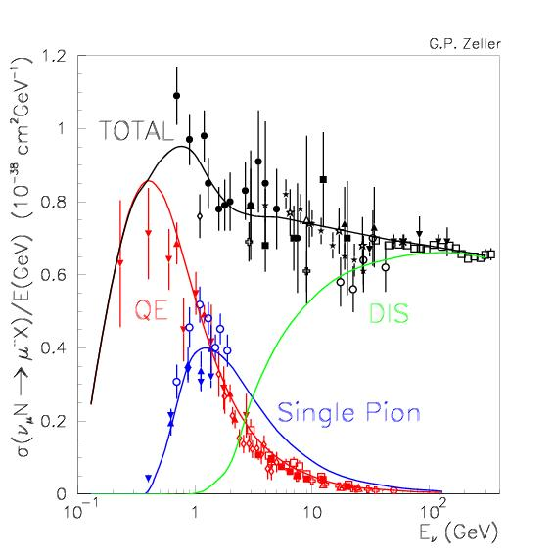
\includegraphics[width=0.9\textwidth]{figures/figs_zeller-total-numode.png}
\caption{Neutrino cross sections, showing the quasi-elastic, deep inelastic and single pion cross sections in the GeV range. Taken from~\cite{82McFarland} modified from original made by G.P.~Zeller~\cite{13PDG} containing data points from various experiments.}
\label{fig:neutrinoInteractionsFig}
\end{figure}

The signature for each of these interactions are quite different as a charge-current quasi-elastic interaction will produce a clean proton and muon track, compared to a shower like pion track or the less clear DIS signature. Baby MIND is designed to operate at a lower energy spectrum, below 5 GeV, meaning that the contribution will be mostly from CCQE and pion interactions. Results from various simulations with the T2K near detector beam spectrum and data recorded from the commissioning will be showed.

%Lab report again, trying to estimate cross-section of interactions. Why? Need it to improve oscillation measurements. Using simulations of muon neutrinos from simulation. What is done, what cuts? How Do we calculate cross-sections? Angular acceptance, look at what Marc has done, do similar things and further the calculations.Discuss what to expect, what kind of interactions could happen in the TASD/WAGASCI? What could be seen? What information? Baby MIND can also have interactions, which ones would be visible? Can reconstruct muons in Baby MIND, electrons and pions visible and potentially reconstructable, but not now. Charge id, momentum. Identifying muons comming of the neutrino interaction with a specific beam and interaction area. Describe the fiducial volume like in my talk for NuFACT.

\section{Muon charge current quasi-elastic}

CCQE interactions produce a clear muon track for both neutrinos and anti-neutrinos, however the interaction only produces a proton track for neutrino interactions as seen below:
\begin{align}
\nu_\mu + n &\rightarrow \mu^- + p\\
 \bar{\nu_\mu} + p &\rightarrow \mu^+ + n
\end{align}

For the neutrino interactions, this becomes a very clear signature in a fully active target where both a muon and proton track can be identified. For anti-neutrinos this is not possible since neutron tracks are usually not detectable for most detector types. However the main goal is to identify muon tracks from pion tracks which is simply identifying a shower from a track. There have been a lot of interesting articles relating to how to identify neutrino events in Argon detectors using machine learning~\cite{83Radovic2018}~\cite{84Adams}. In a non active target it becomes very difficult to identify neutrino interactions as pions may decay to muons and become indistinguishable from directly produced muons.

%Direct simulations with CCQE and different geometries. Use data from specifically Baby MIND in B2 beam line. Explain the beam line etc etc.

%CCQE from muon neutrino produces a muon. Clear production and easy to identify in TASD, not possible in MIND due to the design. 

%Acceptance study, detector layout. Beam settings? Add charge reconstruction, momentum reconstruction. Particle ID? also need interaction ID from TMVA.

%Different size gap, different detector layout both early/testbeam and new at Japan. Cross-section studies. Look at what Marc has done!  Discuss with paul what and how to do cross-section measurements.

\pagebreak
\subsection{Interactions in TASD + Baby MIND}

During the construction of Baby MIND, it was proposed to potentially fully instrument the whole TASD, used during the first beam test, and use it as a fully active target to be combined with Baby MIND, illustrated in~\FigRef{fig:TASDandMIND}.

\begin{figure}[h!]
\centering
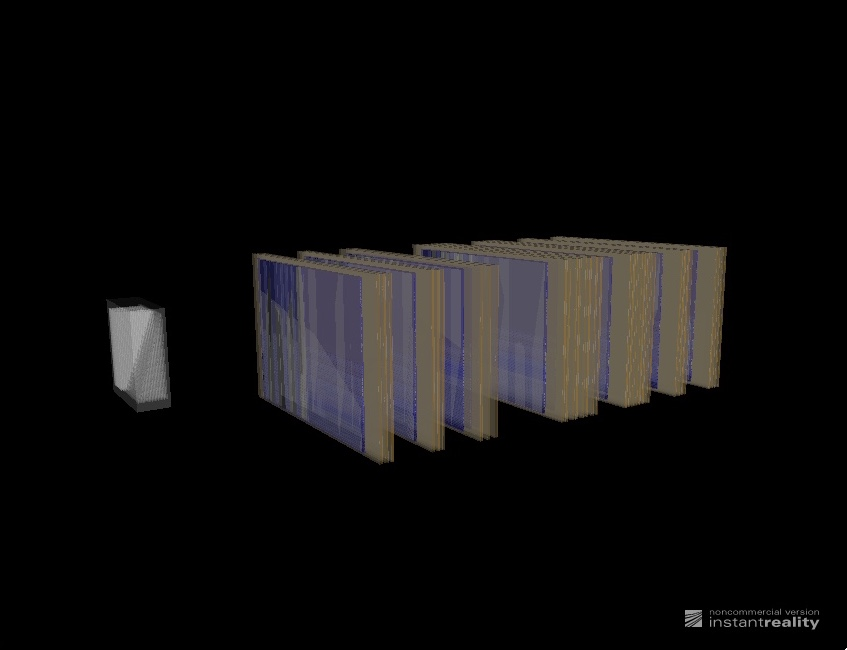
\includegraphics[width=0.9\textwidth]{figures/MINDAida.jpeg}
\caption{An illustrative sketch of the detector setup with the TASD detector in front of Baby MIND.}
\label{fig:TASDandMIND}
\end{figure}

For all analysis the TASD is used as a CCQE identification and neutrino veto, expecting two tracks (neutrino) or atleast start of muon track. The dimentions are the same as mentioned under the test beam section, with a distance of 368mm between the two detectors. Neutrinos are simulated using the T2K near detector spectrum in reverse horn current mode (RHC), seen in~\FigRef{fig:T2KndSpectrum} in the SAURON framework. 



In the framework several figures of merit are produced, the muon energy spectrum, reconstructed muon energy spectrum, reconstructability of tracks vs energy and charge reconstruction vs energy. All of these figures of merit are shown in~\FigRef{fig:T2KTASDfitted} and~\FigRef{fig:T2KTASDfittedcharge}.

\begin{figure}[h!]
\centering
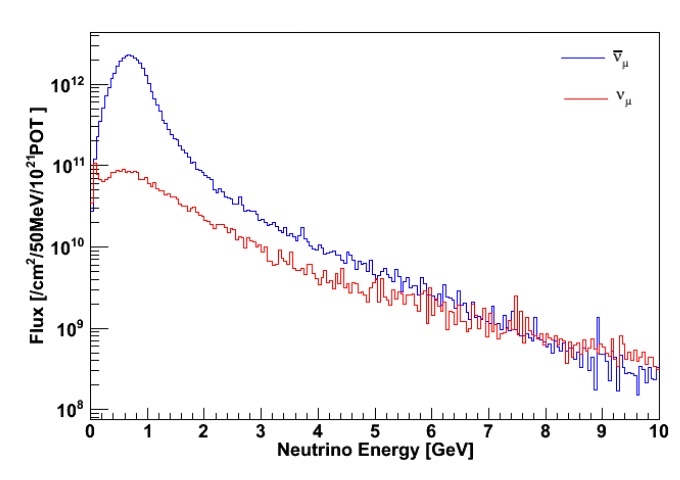
\includegraphics[width=0.9\textwidth]{figures/WAGASCIflux.jpeg}
\caption{The energy spectrum for muon neutrinos and muon anti-neutrinos in the T2K near detector RHC beam.}
\label{fig:T2KndSpectrum}
\end{figure}

\begin{figure}[h!]
\centering
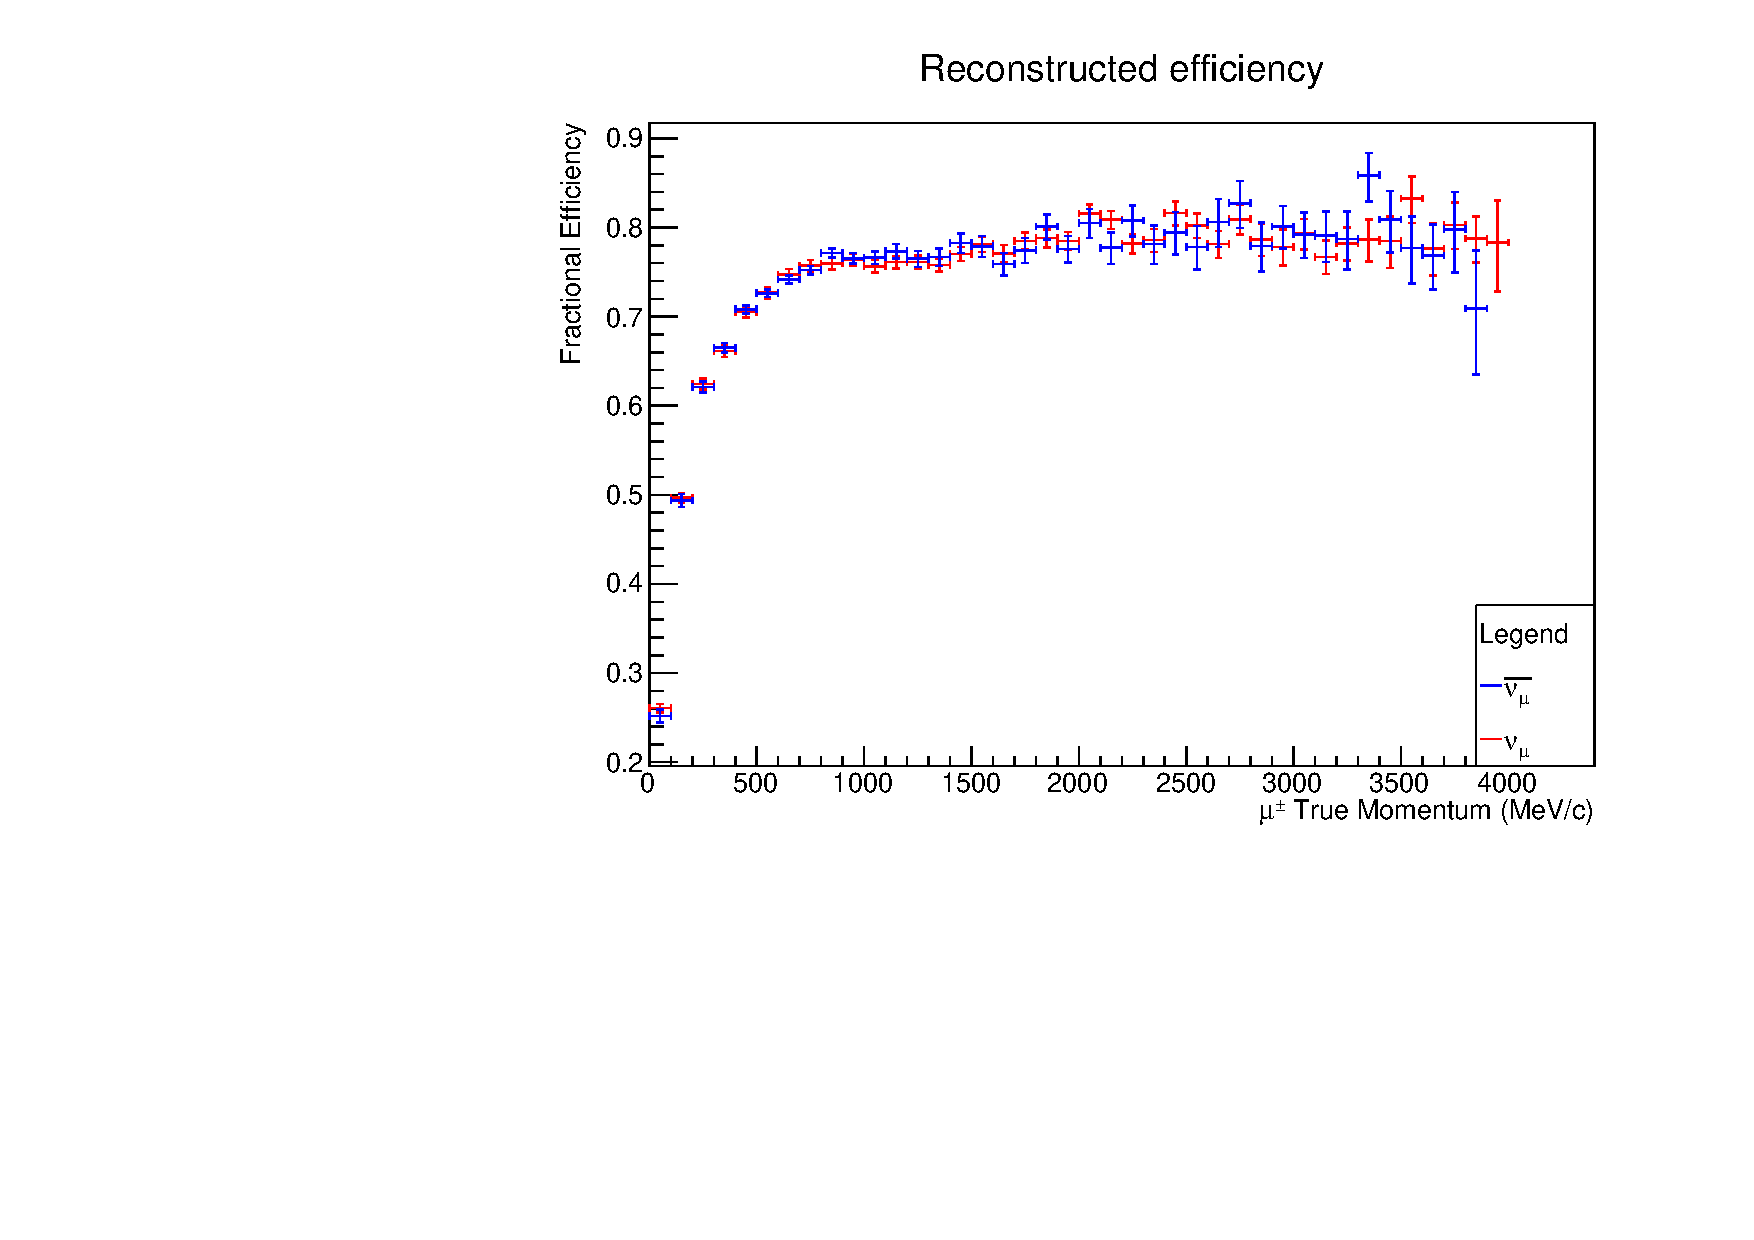
\includegraphics[width=.9\textwidth]{figures/NeutrinoChap/data260618/T2K/FittedT2KNeutrinoBeamMIND.pdf}
\caption{The efficiency plot of how well the algorithm can reconstruct neutrino tracks vs muon momenta for simulated tracks interacting in the TASD.}
\label{fig:T2KTASDfitted}
\end{figure}

\begin{figure}[h!]
\centering
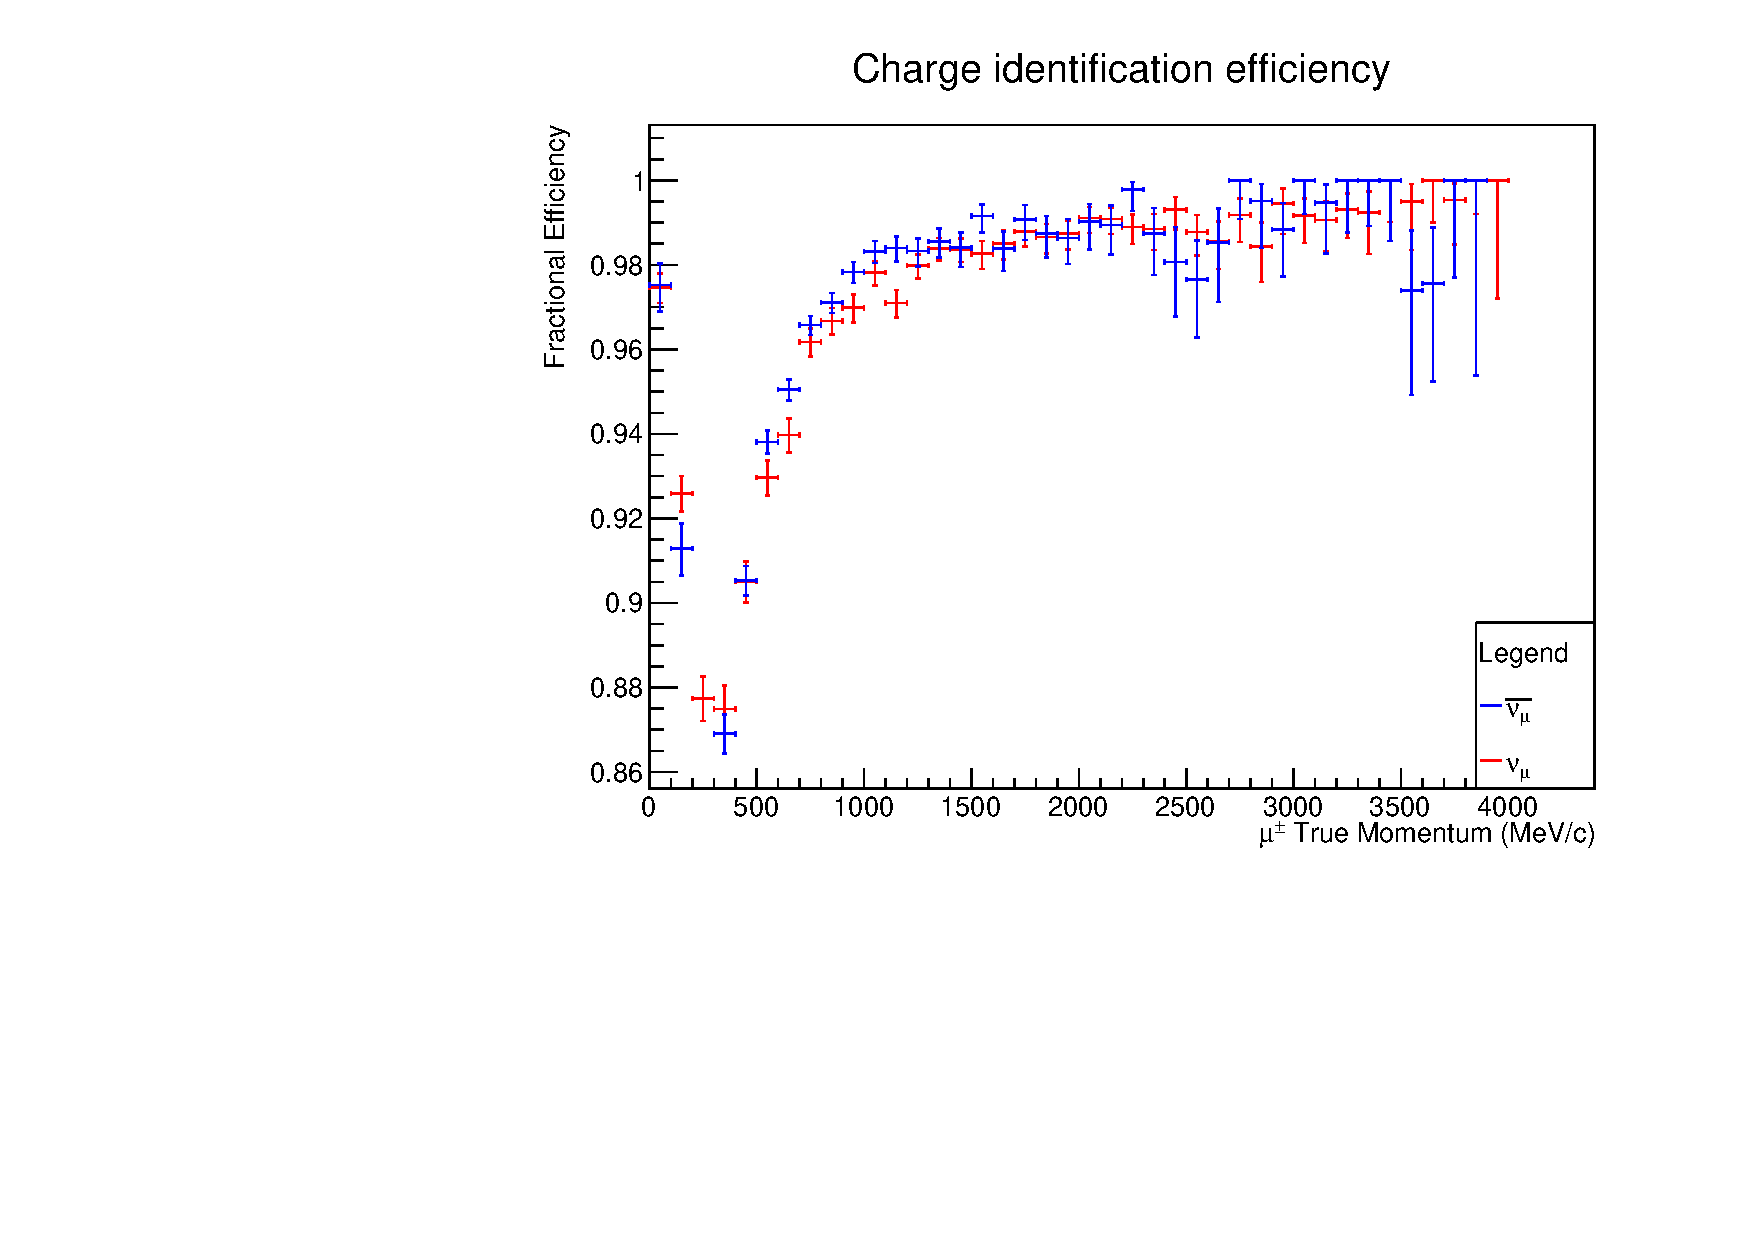
\includegraphics[width=.9\textwidth]{figures/NeutrinoChap/data260618/T2K/ChargeIDT2KNeutrinoBeamMIND.pdf}
\caption{The efficiency plot of how well the algorithm can reconstruct muon charge vs muon momenta for tracks fitted in the algorithm.}
\label{fig:T2KTASDfittedcharge}
\end{figure}





Similarly to the simulated muon beam, and data the charge reconstruction efficiency is very good for the reconstructable tracks. The difference comes from the fact that the neutrinos are produced at angles instead of straight on the center of the detector (with some beam size).Muons from neutrinos are produced at all angles depending on the kinematics of the neutrino interaction and neutrino energy. 


Reshow the muon beam? Discussion about angle etc...



Have simulations both for T2K and NuSTORM beamline, describe both.
Full analysis in MIND, only TASD as veto.
 Shown at NuSTORM talk, fix momentum slightly.
 
\pagebreak
\subsection{Neutrino interactions in Iron in Baby MIND}
Simulations for a  T2K like beam, explain the details and event selection, (None for simulation but easy enough with data). Use the specific fiducial volume. Set up at J-PARC, all the details with that.

To compare simulations with data taken for the commissioning run interactions had to be simulated in the IRON of the Baby MIND due to the fact that the WAGASCI data taking can as of yet not be joined with the Baby MIND data.

\begin{figure}[h!]
\centering
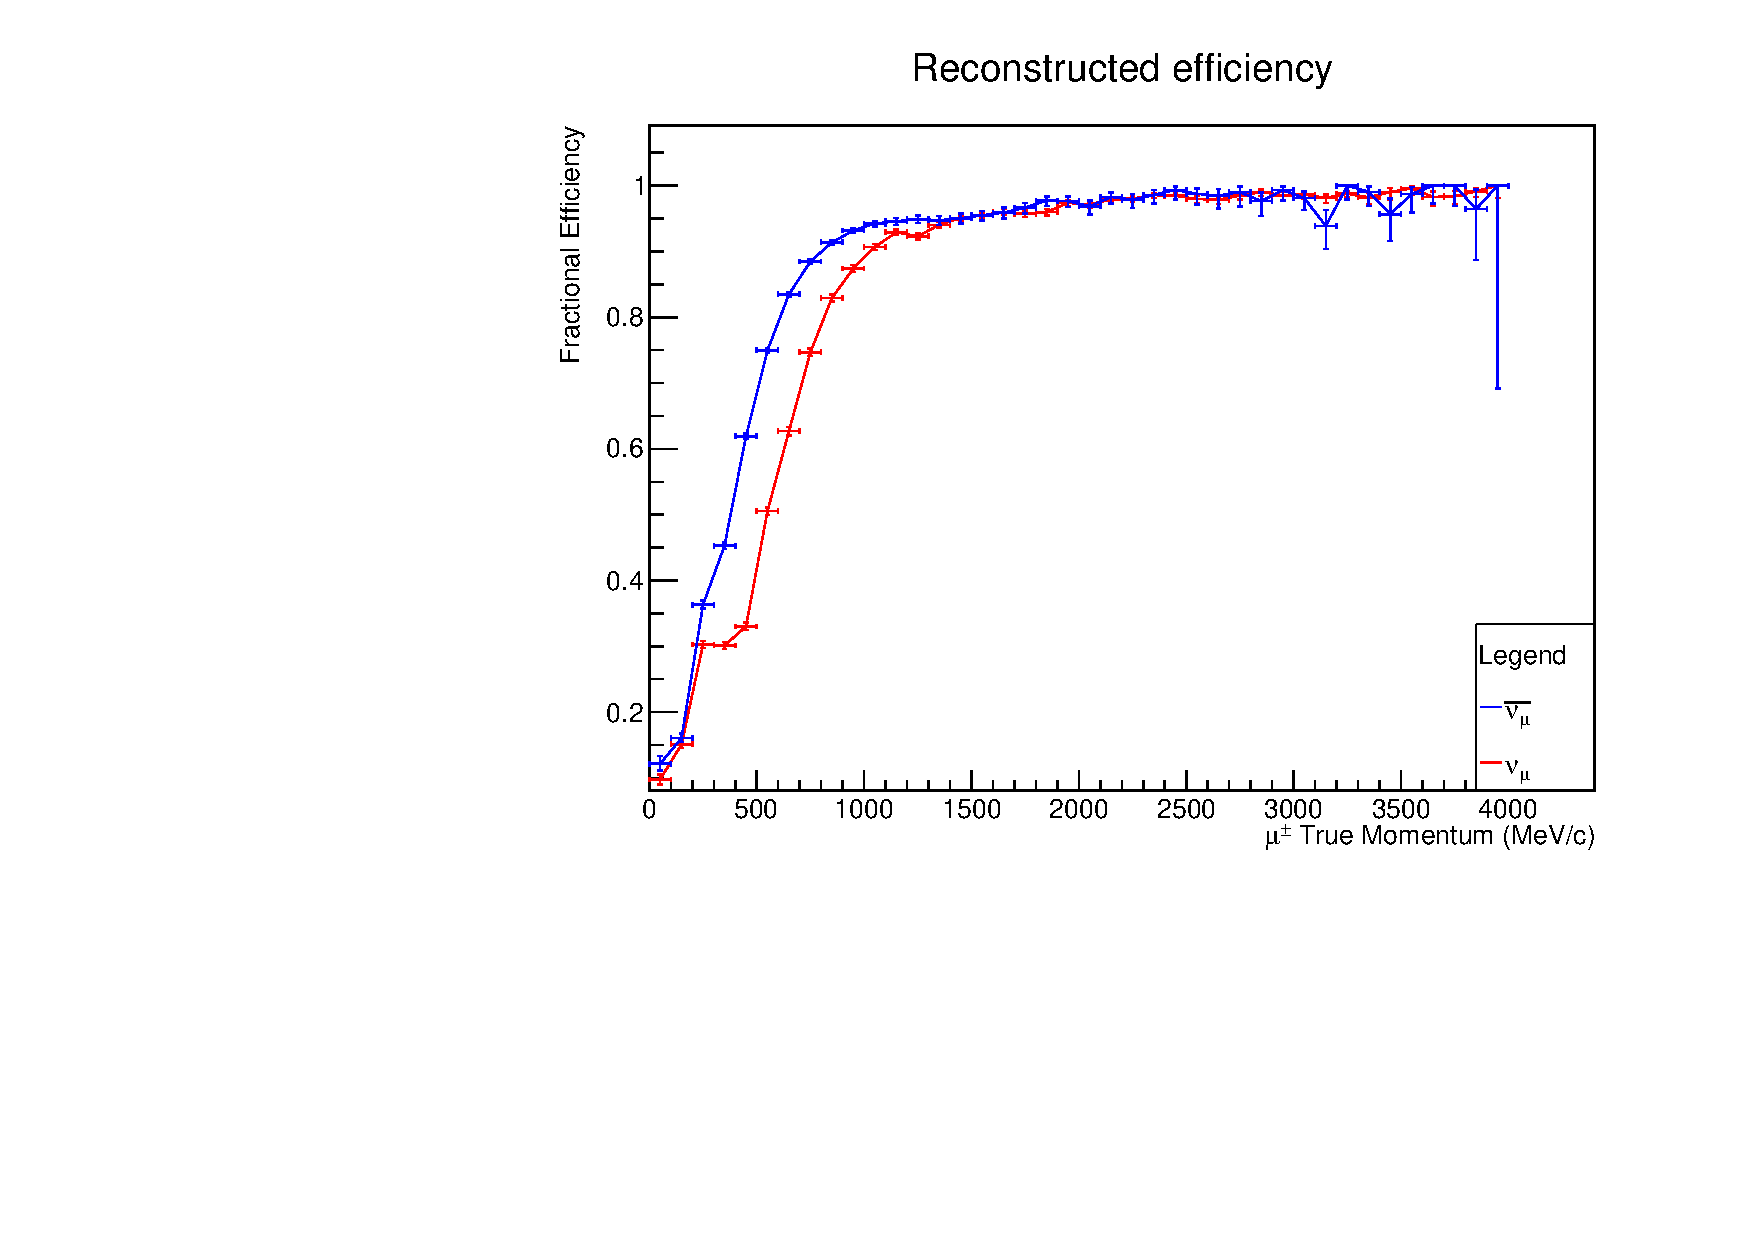
\includegraphics[width=.9\textwidth]{figures/NeutrinoChap/Neutrino/T2KIronRecEff.pdf}
\caption{The efficiency plot of how well the algorithm can reconstruct neutrino tracks vs muon momenta for simulated tracks interacting in the Iron.}
\label{fig:IronMINDfitted}
\end{figure}

\begin{figure}[h!]
\centering
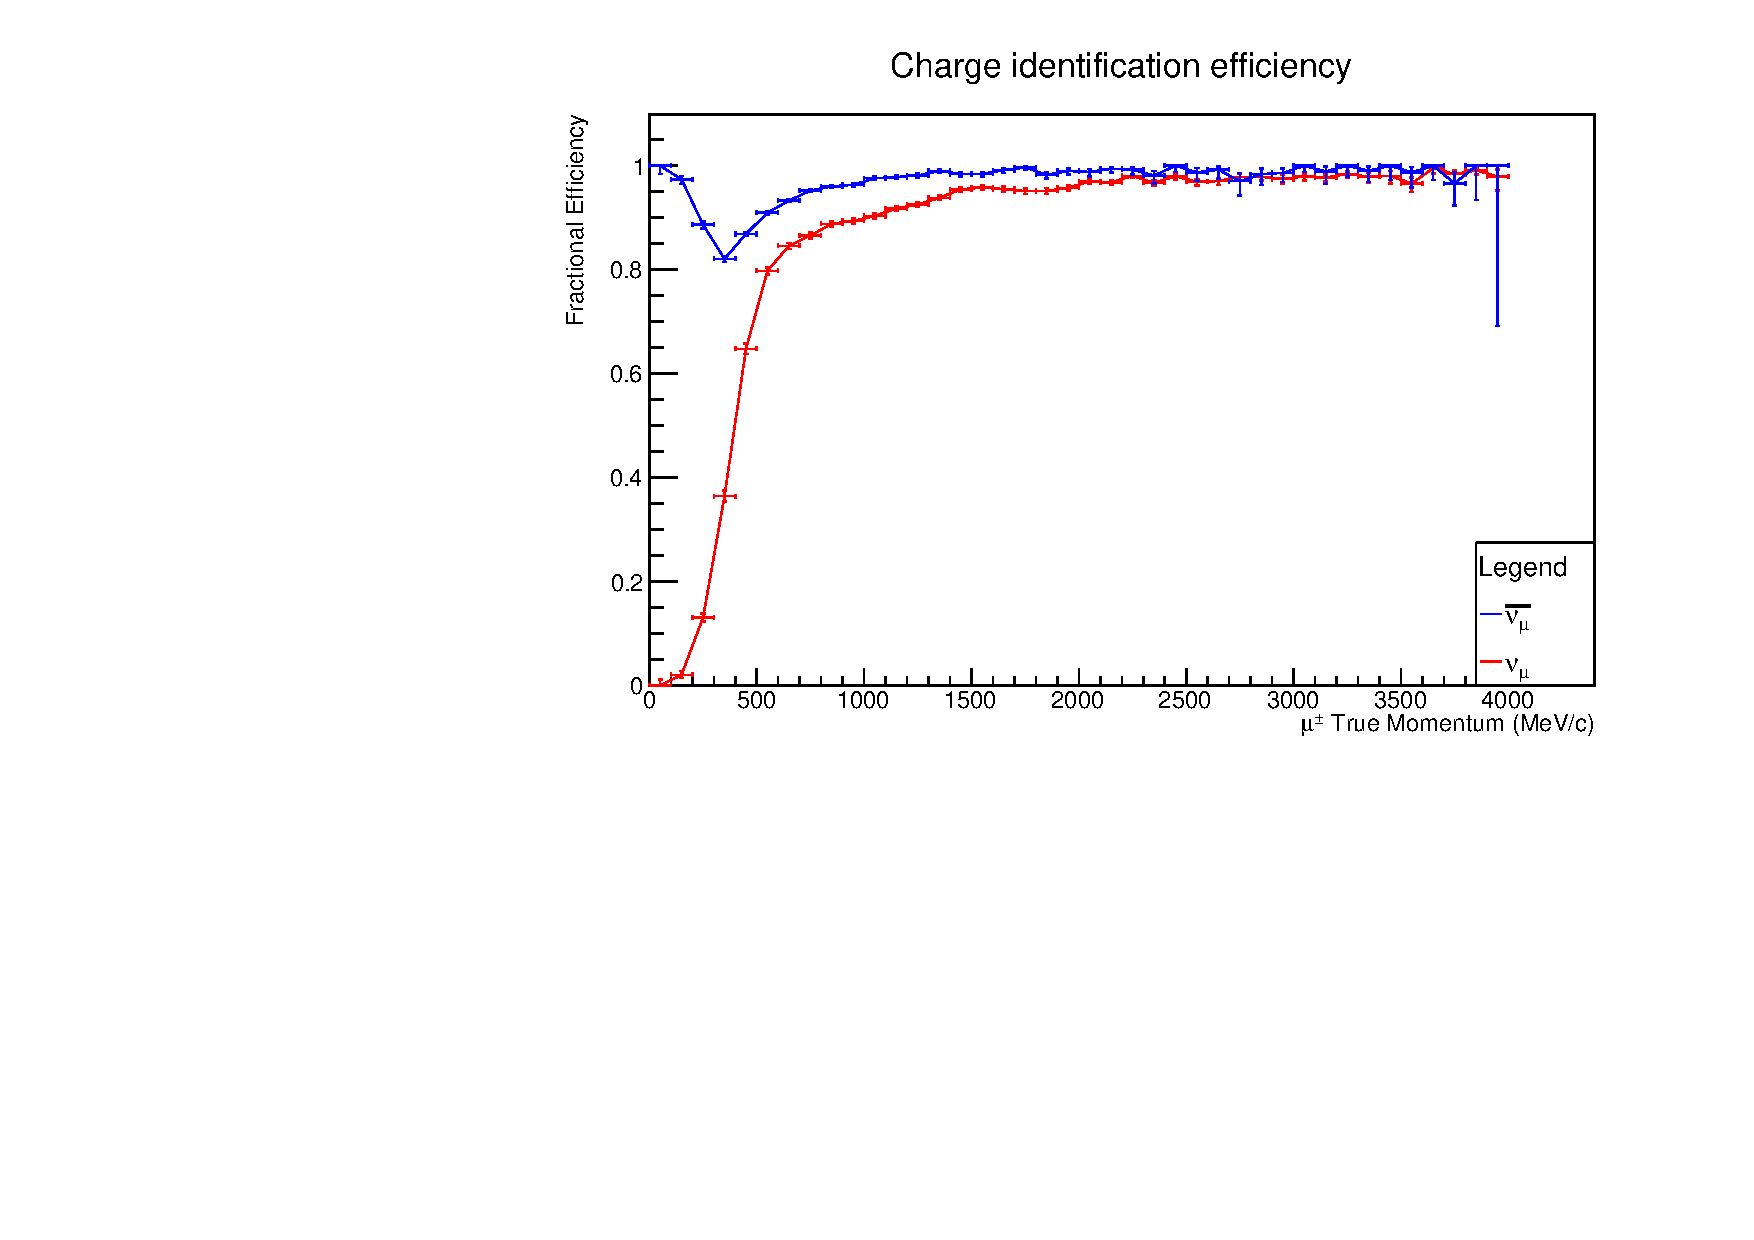
\includegraphics[width=.9\textwidth]{figures/NeutrinoChap/Neutrino/T2KIronChargeEff.pdf}
\caption{The efficiency plot of how well the algorithm can reconstruct muon charge vs muon momenta for tracks fitted in the algorithm.}
\label{fig:IronMINDfittedcharge}
\end{figure}

\pagebreak
\subsubsection{Simulations vs data}
Show same as for nuFact, explain in detail what was done. Show the data.

\pagebreak
\section{Future studies}

\subsection{Neutrino interactions in WAGASCI + Baby MIND}

Using WAGASCI as a CCQE identification,

\subsubsection{Interactions in the full WAGASCI}

Discuss future data taking, interactions everywhere etc etc.

%\subsection{GAr + BabyMIND}
%\subsubsection{Analysis Simulations}
%\subsection{TASD + BabyMIND}
%\subsubsection{Analysis Simulations}
%\subsection{Full WAGASCI}
%\subsubsection{Analysis with Simulations}
%\subsubsection{Simulations vs data}

%\section{Electron charge current quasi-elastic}

